\section{Imágenes Fotoacústicas} \label{sec:intro}

La generación de imágenes utilizando el efecto fotoacústico se ha establecido como una técnica no invasiva valiosa para investigar la composición y estructura de diversos materiales. Este método combina el alto contraste de las imágenes ópticas con la penetración profunda de la detección ultrasónica, lo que lo hace especialmente relevante en aplicaciones biomédicas. El efecto fotoacústico ocurre cuando un material fotoabsorbente absorbe pulsos de luz, lo que genera aumentos localizados de temperatura y, posteriormente, cambios de presión mecánica. Estas ondas de presión se propagan como señales fotoacústicas, las cuales son detectadas por transductores ultrasónicos para crear imágenes.

\begin{figure}[H]
    \centering
    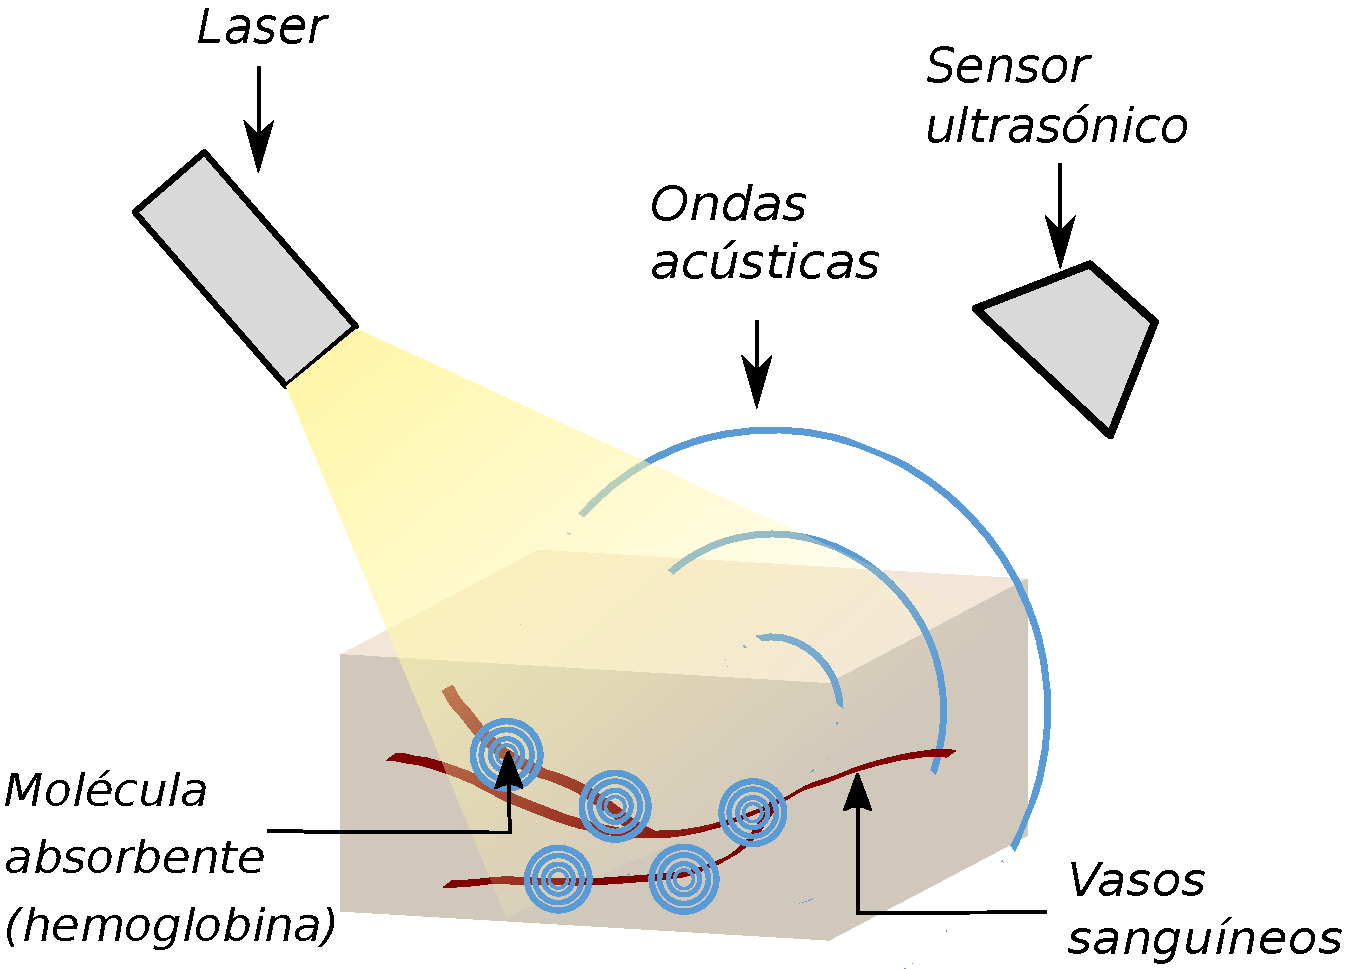
\includegraphics[width=0.6\textwidth]{Images/effect.pdf} 
    \caption{Esquema de imágenes fotoacústicas que muestra cómo el láser y el ultrasonido se combinan para detectar estructuras internas como tumores y vasos sanguíneos.}
    \label{fig:photoacoustic_scheme}
\end{figure}

Las aplicaciones de las imágenes fotoacústicas abarcan diversos campos, con especial importancia en la investigación y el diagnóstico biomédico. Se utilizan ampliamente para evaluar estructuras arteriales, monitorear los niveles de oxigenación tisular, realizar endoscopias gastrointestinales y llevar a cabo imágenes \textit{in vivo} de procesos moleculares y celulares en modelos experimentales. Además, las imágenes fotoacústicas han demostrado ser útiles para estudiar el cerebro y sus funciones en animales, proporcionando información tanto en estados saludables como patológicos.

La reconstrucción de imágenes a partir de señales fotoacústicas requiere un modelado preciso y técnicas computacionales avanzadas. Métodos como la Reversión Temporal, el algoritmo de Retardo y Suma, y las técnicas de Regularización son ampliamente utilizados. Sin embargo, estos métodos enfrentan desafíos debido a la naturaleza mal condicionada del problema de reconstrucción, donde pequeños errores en los datos pueden resultar en grandes desviaciones en las imágenes reconstruidas.

Esta investigación introduce un enfoque novedoso para la reconstrucción de imágenes fotoacústicas, cambiando el enfoque de los métodos tradicionales de regularización hacia la optimización multiobjetivo. Al aprovechar algoritmos evolutivos como \textbf{NSGA-II} y \textbf{MOEA/D}, este enfoque explora un conjunto diverso de soluciones sin la necesidad de predefinir un parámetro de regularización óptimo. La cuidadosa selección de los objetivos permite equilibrar restricciones en competencia, como la precisión, la estabilidad y el realismo físico en el proceso de reconstrucción.

\subsection*{MOEA/D en la Reconstrucción de Imágenes Fotoacústicas}

Además de NSGA-II, esta investigación incorpora \textbf{MOEA/D (Multi-Objective Evolutionary Algorithm based on Decomposition)}, una técnica de optimización multiobjetivo que descompone el problema en múltiples subproblemas escalarizados, cada uno optimizado de manera local. MOEA/D sobresale en escenarios donde se requiere una representación balanceada del frente de Pareto y se deben priorizar soluciones específicas mediante la asignación de pesos.

En este contexto, MOEA/D ofrece las siguientes ventajas para la reconstrucción de imágenes fotoacústicas:
\begin{itemize}
    \item \textbf{Exploración de soluciones balanceadas:} La descomposición del problema asegura que se exploren todas las regiones del frente de Pareto, incluso aquellas menos dominantes.
    \item \textbf{Flexibilidad en la definición de pesos:} Permite priorizar objetivos específicos como la penalización de valores negativos o la regularización, ajustando los pesos de las direcciones de referencia.
    \item \textbf{Mayor robustez frente a ruido:} Las estrategias de vecindario en MOEA/D, junto con la descomposición, mejoran la estabilidad en entornos con ruido.
\end{itemize}

Los experimentos realizados en este estudio destacan cómo MOEA/D complementa a NSGA-II, proporcionando soluciones más balanceadas al incorporar estrategias basadas en pesos. Esto es particularmente relevante en la reconstrucción de imágenes donde el realismo físico y la estabilidad son fundamentales.

\subsection{Preguntas de Investigación} \label{sec:ques}

La naturaleza mal condicionada del problema de reconstrucción en las imágenes fotoacústicas plantea preguntas críticas sobre cómo equilibrar mejor las compensaciones entre precisión, estabilidad y plausibilidad física de las soluciones. Esta investigación busca responder a la siguiente pregunta principal:

\begin{quote}
    \textit{¿Cómo puede la optimización multiobjetivo mejorar la estimación de los parámetros de regularización en la reconstrucción de imágenes fotoacústicas, y cómo se compara esto con los métodos tradicionales como la curva-L?}
\end{quote}

A partir de esta pregunta, el estudio aborda las siguientes subpreguntas:

\begin{enumerate}[start=1,label={RQ\arabic*:},wide = 0pt, leftmargin = 3em]
    \item \textit{¿Cuáles son las limitaciones del método de la curva-L para estimar parámetros de regularización óptimos en la reconstrucción de imágenes fotoacústicas?}
    \item \textit{¿Cómo pueden los algoritmos de optimización multiobjetivo como NSGA-II y MOEA/D mejorar la estimación del parámetro de regularización \( \lambda \)?}
    \item \textit{¿Qué impacto tiene la introducción de objetivos adicionales, como la penalización de la negatividad, en la calidad de las imágenes reconstruidas?}
    \item \textit{¿Cómo se comparan las soluciones obtenidas mediante optimización multiobjetivo en rendimiento e interpretabilidad con las derivadas de métodos tradicionales de un solo objetivo?}
    \item \textit{¿Cómo se desempeña MOEA/D en la estimación de \( \lambda \) frente a NSGA-II y , especialmente en términos de diversidad del frente y calidad de las soluciones reconstruidas?}
\end{enumerate}

\subsection{Contribuciones} \label{sec:cont}

Esta investigación aporta las siguientes contribuciones clave:

\begin{enumerate}[start=1,label={C\arabic*:},wide = 0pt, leftmargin = 3em]
    \item Desarrollo de un marco de optimización multiobjetivo para estimar el parámetro de regularización \( \lambda \) en la reconstrucción de imágenes fotoacústicas.
    \item Introducción y análisis de objetivos adicionales, como la penalización de valores negativos en la solución reconstruida, para mejorar el realismo físico.
    \item Análisis comparativo de las soluciones basadas en algoritmos multiobjetivo frente a los métodos tradicionales de la curva-L, destacando fortalezas y debilidades.
    \item Evaluación integral de frentes de Pareto para visualizar las compensaciones entre objetivos en competencia en la reconstrucción de imágenes.
    \item Implementación de un \textit{pipeline} reproducible para la generación de datos sintéticos y evaluación de métodos de reconstrucción.
    \item Identificación de correlaciones y dependencias entre objetivos de reconstrucción, guiando mejoras algorítmicas futuras.
    \item Integración de MOEA/D como un enfoque complementario para la estimación de \( \lambda \), destacando su capacidad para producir frentes de Pareto balanceados y soluciones robustas frente al ruido.
\end{enumerate}
